\documentclass{article}
\usepackage{tikz}
\usepackage{tkz-euclide}
\usetkzobj{all}
\usetikzlibrary{calc}

\begin{document}



\begin{figure}[h]
\centering
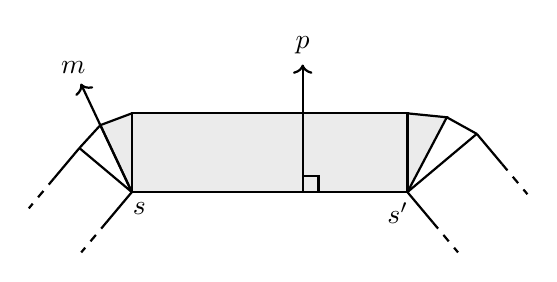
\begin{tikzpicture}

%line info
\def\len{3.5}
\def\theta{50}
\def\w{1}
\def\ratio{1.15}
\def\clenl{0.5}
\def\clenr{0.5}
\def\right{0.2}
%cap points
\coordinate (C)  at (-0.4,\w-0.15);
\coordinate (C') at (\len+0.5,\w-0.05);
%coordinates
\coordinate (B)  at (0,0);
\coordinate (R)  at (0,\w);
\coordinate (B') at (\len,0);
\coordinate (R') at (\len,\w);
\coordinate (N)  at ({-\w/\ratio*sin(\theta)},{\w/\ratio*cos(\theta)});
\coordinate (N') at ({\len+\w*\ratio*sin(\theta)},{\w*\ratio*cos(\theta)});

%fill
\fill[color=black!8!white] (B)  rectangle (R');
\fill[color=black!8!white] (R)  -- (C)  -- (B);
\fill[color=black!8!white] (R') -- (C') -- (B');

%draw edges
\draw[thick] (B)  rectangle (R');
\draw[thick] (B)  -- (N);
\draw[thick] (B') -- (N');
\foreach \x/\y in {0/0,{-\w/\ratio*sin(\theta)}/{\w/\ratio*cos(\theta)}}{
    \draw[thick] ({\x},{\y}) -- ({\x-\clenl*cos(\theta)},{\y-\clenl*sin(\theta)});
    \draw[thick,dashed] ({\x-\clenl*cos(\theta)},{\y-\clenl*sin(\theta)}) -- ({\x-\clenl*2*cos(\theta)},{\y-\clenl*2*sin(\theta)});
}
\foreach \x/\y in {\len/0,{\len+\w*\ratio*sin(\theta)}/{\w*\ratio*cos(\theta)}}{
    \draw[thick] ({\x},{\y}) -- ({\x+\clenr*cos(\theta)},{\y-\clenr*sin(\theta)});
    \draw[thick,dashed] ({\x+\clenr*cos(\theta)},{\y-\clenr*sin(\theta)}) -- ({\x+\clenr*2*cos(\theta)},{\y-\clenr*2*sin(\theta)});
}
\draw[thick] (R)  -- (C)  -- (B)  node[anchor=90+\theta/2]{$s$};
\draw[thick] (R') -- (C') -- (B') node[anchor=90-\theta/2]{$s'$};
\draw[thick] (N)  -- (C);
\draw[thick] (N') -- (C');
%draw arrows
\draw[thick,->] ({0.62*\len},0) -- ({0.62*\len},{1.62*\w}) node[anchor=south]{$p$};
\draw[thick] ({0.62*\len},\right) -- ({0.62*\len+\right},\right) -- ({0.62*\len+\right},0);
\draw[thick,->] (B) -- ($(B)+1.62*(C)$) node[anchor=-90+\theta/2]{$m$};

\end{tikzpicture}
\end{figure}



\begin{figure}[h]
\centering
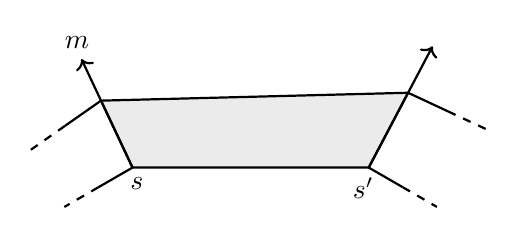
\begin{tikzpicture}

%line info
\def\len{3}
\def\theta{30}
\def\w{1}
\def\ratio{1.15}
\def\clenl{0.5}
\def\clenr{0.5}
\def\right{0.2}
%cap points
\coordinate (C)  at (-0.4,\w-0.15);
\coordinate (C') at (\len+0.5,\w-0.05);
%coordinates
\coordinate (B)  at (0,0);
\coordinate (B') at (\len,0);
\coordinate (N)  at ({-\w/\ratio*sin(\theta)},{\w/\ratio*cos(\theta)});
\coordinate (N') at ({\len+\w*\ratio*sin(\theta)},{\w*\ratio*cos(\theta)});

%fill
\fill[color=black!8!white] (B) -- (C) -- (C') -- (B') -- cycle;

%draw edges
\draw[thick] (B) node[anchor=90+\theta/2]{$s$} -- (C) -- (C') -- (B') node[anchor=90-\theta/2]{$s'$} -- cycle;
\foreach \x/\y [count = \i] in {0/0,{-0.4}/{\w-0.15}}{
    \def\ttheta{\theta+(\i-1)*5}
    \def\tlen{(\clenl+(\i-1)*0.06)}
    \draw[thick] ({\x},{\y}) -- ({\x-\tlen*cos(\ttheta)},{\y-\tlen*sin(\ttheta)});
    \draw[thick,dashed] ({\x-\tlen*cos(\ttheta)},{\y-\tlen*sin(\ttheta)}) -- ({\x-\tlen*2*cos(\ttheta)},{\y-\tlen*2*sin(\ttheta)});
}
\foreach \x/\y [count = \i] in {\len/0,{\len+0.5}/{\w-0.05}}{
    \def\ttheta{\theta-(\i-1)*5}
    \def\tlen{(\clenr+(\i-1)*0.06)}
    \draw[thick] ({\x},{\y}) -- ({\x+\tlen*cos(\ttheta)},{\y-\tlen*sin(\ttheta)});
    \draw[thick,dashed] ({\x+\tlen*cos(\ttheta)},{\y-\tlen*sin(\ttheta)}) -- ({\x+\tlen*2*cos(\ttheta)},{\y-\tlen*2*sin(\ttheta)});
}
%draw arrows
\draw[thick,->] (B)  -- ($(B)+1.62*(C)$) node[anchor=-90+\theta/2]{$m$};
\draw[thick,->] (B') -- ($1.62*(C')-0.62*(B')$);

\end{tikzpicture}
\end{figure}



\begin{figure}[h]
\centering

\begin{tikzpicture}

\pgfmathsetmacro{\square}{0.6}
\pgfmathsetmacro{\cut}{0.7}
\def\cx{-0.25}\def\cy{0.25}
\coordinate (C) at (\cx,\cy);

\draw[thick] (0,0) circle (1.3);
\draw[thick] ($(C)+(\square-\cut,-\square)$) -- ($(C)+(-\square,-\square)$) -- ($(C)+(-\square,\square)$) -- ($(C)+(\square,\square)$) -- ($(C)+(\square,-\square+\cut)$);

\tkzDefPoint(\square-\cut+\cx,-\square+\cy){A1}\tkzDefPoint(\cx,\cy){A2}\tkzDefPoint(\square+\cx,-\square+\cut+\cy){A3}
\tkzCircumCenter(A1,A2,A3)\tkzGetPoint{AC}
\tkzDrawArc[thick,color=black](AC,A3)(A1)

\end{tikzpicture}
\end{figure}



\end{document}
